\chapter{Ενεργοί γαλαξιακοί πυρήνες} 

Οι ενεργοί γαλαξίες και οι ενεργοί γαλαξιακοί πυρήνες (\textlatin{AGN}) διαφέρουν από απλούς, μη-ενεργούς γαλαξίες στο ότι στο κέντρο τους υπάρχει μία υπερμεγέθης μελανή οπή (\textlatin{Supermassive Black Hole - SMBH}) η οποία βρίσκεται σε διαδικασία προσαύξησης. Εκτιμάται ότι στο τοπικό σύμπαν ($z \leq 0.1$) ένας στους 50 γαλαξίες περιέχει υπερμεγέθη μελανή οπή με γρήγορο ρυθμό προσαύξησης και περίπου ένας στους 3 γαλαξίες περιέχει υπερμεγέθη μελανή οπή με αργό ρυθμό προσαύξησης\cite{netzer_2013}.

Οι \textlatin{AGN} χωρίζονται σε δύο γενικές κατηγορίες βάσει παρατηρησιακών κριτιρίων: \textlatin{AGN} τύπου Ι για πηγές με καθαρή, διακριτή γραμμή παρατήρησης \textlatin{(line-of-sight)} έως το κέντρο τους kai \textlatin{AGN} τύπου ΙΙ για αντικείμενα με αδιόρατη γραμμή παρατήρησης, σκιασμένη σε βαθμό ώστε σχεδόν όλη η ακτινοβολία στο οπτικό και υπεριώδες από την κεντρική περιοχή ακτίνας ενός \textlatin{parsec} να έχει απορροφηθεί. \\
Διακρίνουμε τους \textlatin{AGN} βάσει παρατηρησιακών τους χαρακτηριστικών όπως βολομετρική λαμπρότητα $ L_{bol}$, επίπεδο ιονισμού του αερίου στο οποίο οφείλεται το γραμμικό φάσμα εκπομπής, το εύρος των φασματικών γραμμών εκπομπής ή/και απορρόφησης και την ένταση της πηγής μη-θερμικής ακτινοβολίας. Ο ορισμός δραστηριότητας του πυρήνα ενός γαλαξία μπορεί να βασιστεί είτε στον φυσικό μηχανισμό είτε στα παρατηρησιακά χαρακτηριστικά της δραστηριότητας. Ο ορισμός βάσει φυσικού μηχανισμού είναι απλός- ένα εξωγαλαξιακό αντικείμενο που περιέχει υπερμεγέθη μελανή οπή στο κέντρο του η οποία προσαυξάνεται θεωρείται \textlatin{AGN}. Η παρατηρησιακή ταξινόμηση δεν είναι πάντα τόσο ξεκάθαρη λόγω περιορισμών όπως σκίαση \textlatin{(obscuration)} της πηγής, και επειδή με τον όρο <<δραστηριότητα>> καλύπτουμε πολλές τάξεις μεγέθους ρυθμού προσαύξησης. Συχνά, λοιπόν, ένα εξωγαλαξιακό αντικείμενο χαρακτηρίζεται \textlatin{AGN} αν τουλάχιστον ένα από τα παρακάτω παρατηρησιακά κριτήρια πληρούνται\cite{netzer_2013}:
\begin{itemize}
    \item Περιέχει μια συμπαγή κεντρική περιοχή που εκπέμπει σημαντικά περισσότερο απ> ότι είναι αναμενόμενο από αστρικές διαδικασίες που αντιστοιχούν στον συγκεκριμένο τύπο γαλαξία.
    \item Εκπέμπει στο συνεχές από το κέντρο του από μη-αστρικές διαδικασίες.
    \item Το φάσμα του περιέχει έντονες γραμμές εκπομπής και οι αναλογίες γραμμών είναι τυπικές για μη-αστρικό πεδίο ακτινοβολίας.
    \item Υπάρχουν μεταβολές στο γραμμικό ή/και στο συνεχές φάσμα.
\end{itemize}
%\section{Βασικές παρατηρούμενες ιδιότητες των \textlatin{AGN} }
Βασικές παρατηρούμενες ιδιότητες των \textlatin{AGN} είναι η εκπομπη σε όλο το ενεργειακό φασμα, η παρουσία γραμμών εκπομπής (ευρείες ή στενές) καθώς και η μεταβλητότητα στο φάσμα (τόσο στο συνεχές όσο και στο γραμμικό).

\section{Εκπομπή σε όλο το ηλεκτρομαγνητικό φάσμα}

Το φάσμα των \textlatin{AGN} είναι χαρακτηριστικό σε πολλά διαφορετικά μήκη κύματος. Χρησιμοποιούμε την συνάρτηση κατανομής φασματικής ενέργειας (\textlatin{SED}) για να το περιγράψουμε με όρους μονοχρωματικής λαμπρότητας ανά συχνότητα ($L_\nu$, που μετράται σε \textlatin{erg s}$^{-1}$ \textlatin{Hz}$^{-1}$) ή ανά ενέργεια ($L_E$, που μετράται σε \textlatin{erg s}$^{-1}$ \textlatin{erg}$^{-1}$) ή ανά μήκος κύματος ($L_\lambda$, που μετράται σε \textlatin{erg s}$^{-1}$ \AA$^{-1}$). Oi αντίστοιχες μονοχρωματικές ροές ($F_\nu$, $F_E$, $F_\lambda$) είναι οι παραπάνω ποσότητες ανά μονάδα επιφάνειας (παράγοντας μονάδων  \textlatin{cm}$^{-2}$) και χρησιμοποιούνται για να περιγράψουν τις παρατηρούμενες ιδιότητες. Η μετατροπή της \textlatin{SED} με βάση την συχνότητα σε \textlatin{SED} με βάση το μήκος κύματος γίνεται από την διατήρηση ενέργειας: $$ L_\nu d\nu  = L_\lambda d\lambda$$
Στην αστρονομία ακτίνων Χ χρησιμοποιείται και η ποσότητα ρυθμού φωτονίων (\textlatin{count rate})\cite{netzer_2013}. Ο ρυθμός φωτονίων είναι μία παρατηρούμενη ιδιότητα της πηγής, ενώ οι μονοχρωματικές ροές είναι ενδογενείς ιδιότητες που προκπτουν από την λαμπρότητα της πηγής.
%υπαρχει μια διαφορα αναμεσα στα προηγουμενα και στο ρυθμο φωτονιων, ο τελευταιος ειναι παρατηρουμε ιδιοτητα (ροη) σε αντιθεση με τα προηγουμενα που αναφερονται σε ενδογεννεις ιδιοτητες (φωτηνοτητες).

\subsection*{Παρατηρήσεις στο οπτικό και υπεριώδες}

Οι εικόνες \textlatin{AGN} τύπου Ι στο οπτικό δείχνουν σημειακές κεντρικές πηγές με εκπομπή σημαντικά περισσότερη της περιβάλουσας του αστρικού υποβάθρου του γαλαξία. Η προέλευση της ακτινοβολίας του συνεχούς φασματος θεωρείται ότι είναι ακτινοβολία μελανού σώματος (θερμική) αστρικής προέλευσης,  ακτινοβολία μελανού σώματος μη-αστρικής προέλευσης και ένα μικρό ποσοστό ακτινοβολίας από διαδικασίες \textlatin{Compton} μη-αστρικής προέλευσης. Η μη-αστρική προέλευση της ακτινοβολίας αυτών των πηγών καθορίζεται από το σχημα της \textlatin{SED} τους kai από την απουσία έντονων γραμμών απορρόφησης (τυπικές αστρικού φάσματος). Συγκεκριμένα, το συνεχές φάσμα είναι νόμος δύναμης (υπέρθεση πολλών θερμικών φασμάτων) και θεωρείται ότι προέρχεται από δίσκο προσάυξησης. Οι \textlatin{AGN} τύπου ΙΙ, είναι σχεδόν αδιόρατοι στο οπτικό και δεν εμφανίζουν αυτήν την πλεονάζουσα κεντρική εκπομπή.\\ 
Το φάσμα στο οπτικό και υπεριώδες \textlatin{(UV)} είναι αυτό που μας βοηθά να κάνουμε τον διαχωρισμό πηγών τύπου Ι και ΙΙ με υψηλό ιονισμό από πηγές Ι και ΙΙ με χαμηλό ιονισμό του αερίου του φάσματος εκπομπής, καθώς οι γραμμές διαφόρων βαθμών ιονισμού των πιο κοινών στοιχείων βρίσκονται σε αυτό το εύρος μηκών κύματος ($900-7000$ \AA). 
Οι \textlatin{AGN} τύπου ΙΙ παρουσιάζουν στενές γραμμές εκπομπής με πλήρες πλάτος στο ήμισυ του μέγιστου ύψους (\textlatin{FWHM}) να παίρνει τιμές $400-800$ \textlatin{km  s}$^{-1}$
ενώ οι \textlatin{AGN} τύπου Ι έχουν ευρύτερες γραμμές εκπομπής με \textlatin{FWHM} που υποδηλώνει ταχύτητες αερίων μέχρι και $5000 - 10000$ \textlatin{km  s}$^{-1}$, αν θεωρήσουμε ότι το πλάτος των φασματικών γραμμών οφείλεται κυρίως σε κίνηση \textlatin{Doppler.} Η πληροφορία της κινηματικής αερίων από την περιοχή εκπομπής ευρείων φασματικών γραμμών \textlatin{(BLR)} στους \textlatin{AGN} τύπου Ι (η οποία είναι πολύ κοντά στην κεντρική μελανή οπή) χρησιμεύει ώστε να υπολογίσουμε απ> ευθείας την μάζα της \textlatin{SMBH}\cite{netzer_2013}.\\
Ο όρος <<vευρείες γραμμές εκπομπής>> που χρησιμοποιείται για να περιγράψει επιτρεπτές και ημιαπαγορευμένες γραμμές εκπομπής σε \textlatin{AGN} τύπου Ι δεν υποδηλώνει παρόμοια πλάτη όλων των γραμμών σε όλες τις πηγές. Οι διαφορετικές ευρείες γραμμές εκπομπής έχουν διαφορετικά πλάτη και σε γενικές γραμμές στο πλάτος αυτό αντικατοπτρίζεται ο βαθμός ιονισμού του αερίου, η λαμπρότητα της πηγής και η μάζα κεντρικής μελανής οπής.

%φυσικες διαδικασιες: πιστευουμε οτι το συνεχες προερχεται απο το δισκο προσαυξησης. Επισης ειναι νομος δυναμης στο συνεχες (πχ υπερθεση πολλων θερμικων φασματων)

\subsection*{Παρατηρήσεις στο υπέρυθρο και μακρυνό υπέρυθρο}

Οι παρατηρήσεις σε μήκη κύματος $0.3$ m\textlatin{m} $- 1.2$ \textlatin{mm} μπορούν να χωριστούν στις κατηγορίες: κοντινό υπέρυθρο (\textlatin{near infrared- NIR}, περίπου $0.3-3.5$ m\textlatin{m}), μέσο υπέρυθρο (\textlatin{mid infrared- MIR}, περίπου $3.5- 10$ m\textlatin{m}), μακρυνό υπέρυθρο (\textlatin{far infrared- FIR}, περίπου $10-400$ m\textlatin{m}) kai υπο-χιλιοστομετρικές παρατηρήσεις (\textlatin{sub-millimetre}, περίπου $0.4-1.2$ \textlatin{mm}).\\
Παρατηρήσεις στο κοντινό υπέρυθρο μας δίνουν φωτομετρία και φασματοσκοπία \textlatin{J} (στα μήκη κύματος $\sim 1.2$ m\textlatin{m}), \textlatin{H} (στα μήκη κύματος $\sim 1.6$ m\textlatin{m}), \textlatin{K} (στα μήκη κύματος $\sim 2.2$ m\textlatin{m}) kai \textlatin{L} (στα μήκη κύματος $\sim 3.5$ m\textlatin{m}).\\
Οι παρατηρήσεις στο μέσο υπέρυθρο γίνονται και με διαστημικά τηλεσκόπια αλλά και από την Γη (για κοντινές πηγές- δηλαδή για πολύ λαμπρές πηγές) και μας δίνουν φωτομετρία και φασματοσκοπία \textlatin{Ν} (στα μήκη κύματος $\sim 10$ m\textlatin{m}). Οι υδρατμοί στην γήινη ατμόσφαιρα απορροφούν ορισμένα μήκη κύματος στο κοντινό και μέσο υπέρυθρο ενώ απορροφούν σχεδόν ολοκληρωτικά το μακρυνό υπέρυθρο και τα υποχιλιοστομετρικά μήκη κύματος, επίσης η Γη εκπέμπει στο υπέρυθρο- έτσι τα επίγεια τηλεσκόπια βρίσκονται σε περιοχές με χαμηλή υγρασία και υψηλό υψόμετρο και στα παράθυρα που επιτρέπονται από την γήινη ατμόσφαιρα. Οι παρατηρήσεις στο μακρυνό υπέρυθρο γίνονται και με διαστημικά τηλεσκόπια (με πολύ καλή χωρική διακριτότητα και για ερυθρομετατοπίσεις μέχρι 5 και μεγαλύτερες) αλλά και από την Γη. Οι υπο-χιλιοστομετρικές παρατηρήσεις γίνονται από επίγεια παρατηρητήρια για \textlatin{AGN} μέχρι πολύ μεγάλες ερυθρομετατοπίσεις.\\
Η εκπομπή ακτινοβολίας στο κοντινό και στο μέσο υπέρυθρο οφείλεται σε δευτερογενή θερμική εκπομπή από σκόνη που αντιστοιχεί σε θερμοκρασίες $100-2000$ K (<<δευτερογενή>> εκπομπή εννοούμε εκπομπή από θερμούς ή ψυχρούς κόκκους σκόνης που θερμαίνονται από την πρωτογενή πηγή ακτινοβολίας του \textlatin{AGN}- <<πρωτογενή>> εκπομπή εννοούμε την ακτινοβολία που είναι άμεσο αποτέλεσμα της διαδικασίας προσαύξησης). Οι διαστάσεις της περιοχής της σκόνης που εκπέμπει την ακτινοβολία αυτή για \textlatin{AGN} μέσης λαμπρότητας είναι της τάξης του ενός \textlatin{parsec}. Το μεγαλύτερο ποσό της θερμικής ακτινοβολίας μακρυνού υπερύθρου θεωρείται ότι οφείλεται σε ψυχρότερη σκόνη που θερμαίνεται από νεαρά άστρα σε μεγάλες περιοχές αστρογένεσης του γαλαξία, ενώ για τις πηγές που εκπέμπουν ισχυρά στα ραδιοκύματα μέρος της ακτινοβολίας μακρυνού υπερύθρου οφείλεται σε μή θερμικές διαδικασίες που λαμβάνουν χώρα σε περιοχές κοντυνότερες στον γαλαξιακό πυρήνα (επιτάχυνση φορτισμένων σωματιδίων σε μαγνητικά πεδία- ακτινοβολία σύγχροτρον). Στο φάσμα πολλών \textlatin{AGN} παρατηρούνται ευρείες και στενές γραμμές εκπομπής στο υπέρυθρο. Συνολικά, για το φάσμα σε μήκη κύματος $0.3 -30$ m\textlatin{m} ενός \textlatin{AGN} τύπου Ι μέσης λαμπρότητας, η εκπομπή από $0.3$ m\textlatin{m} έως $1 $ m\textlatin{m}  οφείλεται σε δευτερογενή θερμική ακτινοβολία από σκόνη. Περίπου στο $1$ m\textlatin{m} η φασματική ενέργεια παρουσιάζει πτώση επειδή ελαττώνεται το συνεχές φάσμα που παράγεται από τον δίσκο στα μικρά μήκη κύματος και από τα $1$ m\textlatin{m} η φασματική ενέργεια επανέρχεται λόγω ακπομπής από θερμή σκόνη και παρατηρούνται αυξημένες ροές στα $\sim 10 $ m\textlatin{m} kai $\sim 18$ m\textlatin{m} χαρακτηριστικές πυριτικών ανιόντων\cite{netzer_2013}.

\subsection*{Παρατηρήσεις στα ραδιοκύματα}

Η ανακάλυψη των πρώτων ραδιογαλαξιών έγινε πριν την οπτική ανακάλυψη των πρώτων \textlatin{AGN}. Τα κύρια χαρακτηριστικά των ενεργών αυτών γαλαξιακών πυρήνων είναι η ύπαρξη μονών ή διπλών λοβών διαστάσεων πολύ μεγαλύτερων του γαλαξία στον οποίο βρίσκονται, ισχυροί ραδιο-πυρήνες και (σε μερικές πηγές) ραδιο-πίδακες που συμπίπτουν με την θέση του γαλαξιακού πυρήνα στο οπτικό. Η συνεχής εκπομπή ραδιοκυμάτων από τους \textlatin{AGN} οφείλεται κυρίως σε διαδικασίες ακτινοβολίας σύγχροτρον και \textlatin{bremsstrahlung} και φαίνεται να συσχετίζεται περισσότερο με τους πίδακες των ενεργών γαλαξιακών πυρήνων και να μην σχετίζεται άμεσα με την προσάυξηση στην κεντρική μελανή οπή\cite{Radcliffe}.\\   
Οι περισσότεροι \textlatin{AGN} έχουν κάποια εκπομπή στα ραδιοκύματα, όμως φαίνεται πως υπάρχουν δύο διακριτές κατηγορίες \textlatin{AGN} βάσει της ιδιότητας αυτής. Διαχωρίζουμε τους \textlatin{AGN} σε ραδιοϊσχυρούς \textlatin{(radio-loud)} και ραδιοήσυχους \textlatin{(radio-quiet)} ορίζοντας παράμετρο $R$ η οποία δίνει ένα μέτρο της αναλογίας μονοχρωματικής λαμπρότητας στα ραδιοκύματα ($5$ \textlatin{GHz}) πρός την μονοχρωματική λαμπρότητα στο οπτικό (\textlatin{B-band}):
$$ R = \dfrac{L_\nu(5\;GHz)}{L_\nu (4400\;\AA)} = 1.36 \times 10^{5} \;\dfrac{L(5\;GHz)}{L (4400\;\AA)} $$
Όπου $L$(5 \textlatin{GHz}) και $L$(4400 \textlatin{GHz}) είναι η ποσότητα $\lambda \cdot L_\lambda$ στα αντίστοιχα μήκη κύματος. Η διαχωριστική γραμμή μεταξύ ραδιοϊσχυρών και ραδιοήσυχων συνήθως είναι η $R=10$. Περίπου 10\% των \textlatin{AGN} που έχουν παρατηρηθεί είναι ραδιοϊσχυροί, ενώ υπάρχουν ενδείξεις ότι το ποσοστό αυτό φθίνει με την ερυθρομετατόπιση. \\
Στούς ραδιοϊσχυρούς \textlatin{AGN} παρατηρούμε ραδιοπηγές με κυρίαρχη ραδιοακτινοβολία από τον πυρήνα \textlatin{(core-dominated)} και ραδιοπηγές με κυρίαρχη ραδιοακτινοβολία από τους λοβούς \textlatin{(lobe-dominated)}. Οι διαφορές αυτών των δύο αντικατοπτρίζεται και στην μορφή του φάσματός τους, ενώ οι \textlatin{lobe-dominated} παρουσιάζουν πολύ μικρότερη μεταβλητότητα\cite{netzer_2013}.

\subsection*{Παρατηρήσεις στις ακτίνες Χ}

Παρατηρήσεις στις ακτίνες Χ ($0.2-100$ \textlatin{keV}) πραγματοποιούνται από διαστημικά τηλεσκόπια με κύριες ενεργειακές κατηγορίες τις μαλακές ακτίνες Χ $0.2-2$ \textlatin{keV} και τις σκληρές ακτίνες Χ $2-10$ \textlatin{keV}. Οι \textlatin{AGN} στις ακτίνες Χ εμφανίζονται ως σημειακές πηγές (οι τύπου Ι σε όλες τις ενέργειες, ενώ οι τύπου ΙΙ μόνο σε σκληρές ακτίνες Χ). 
Το φάσμα μαλακών ακτίνων Χ των \textlatin{AGN} τύπου Ι εμφανίζει πολλές στενές γραμμές απορρόφησης σε ένα ισχυρό συνεχές φάσμα ακτίνων Χ- οι απορροφητές είναι υλικό που βρίσκεται στην γραμμή παρατήρησής μας. Στους \textlatin{AGN} τύπου ΙΙ παρατηρούνται στενές γραμμές εκπομπής οι οποίες συσχετίζονται με τις ισχυρότερες γραμμές απορρόφησης- οι τελευταίες οφείλονται στο μέσο σκίασης της γραμμής παρατήρησής μας. Η βασική διαφορά, όμως, μεταξύ \textlatin{AGN} τύπου Ι και τύπου ΙΙ στις ακτίνες Χ είναι στο συνεχές φάσμα καθώς στους \textlatin{AGN} τύπου ΙΙ αυτό απορροφάται.\\
Στην αστρονομία ακτίνων Χ χρησημοποιείται ο αριθμός φωτονίων ανά μονάδα χρόνου ανά ενέργεια $Ν(Ε)$ αντί της ροής μονοχρωματικής λαμπρότητας $L$. 
Η κλίση ενεργειακού φάσματος $\alpha_{ox}$ χρησιμοποιείται για να συγκρίνει ποσοτικά την λαμπρότητα \textlatin{AGN} τύπου Ι στο οπτικό και υπεριώδες με αυτήν στις ακτίνες Χ, μελέτη αυτού του χαρακτηριστικού μας οδηγεί στο συμπέρασμα ότι ακόμα και στους λαμπρότερους \textlatin{AGN}, η λαμπρότητα στις ακτίνες Χ είναι ένα μικρό κλάσμα της βολομετρικής του \textlatin{AGN}.\\
Οι διαδικασίες ακτινοβολίας από τις οποίες προκύπτει φάσμα ακτίνων Χ είναι αντίστροφος σκεδασμός \textlatin{Compton} (σχετικιστικά ηλεκτρόνια σκεδάζουν φωτόνια αυξάνοντας την ενέργεια των φωτονίων αυτών) και ακτινοβολία πέδης \textlatin{bremsstrahlung}- και οι δύο αυτές διαδικασίες δίνουν χαρακτηριστικό φάσμα νόμου δύναμης, όπως θα δούμε και στο επόμενο κεφάλαιο.
%Η βασικη διαφορα αναμεσα σε τυπου Ι και ΙΙ στις ακτινες-Χ ειναι το συνεχες, που απορροφαται στα τυπου δυο. Οι γραμμες εκμπομπης/απορροφησης δεν ακολουθουν το οπτικο καθως οι φυσικες διαδικασιες παραγωγης ειναι διαφορετικες. Η πλεον ισχυση γραμμη εκπομπης στις ακτινες, Fe-Ka, εμφανιοζεται (μερικες φορες) φαρδυα λογω βρατυρικων φαινομενων και οχι επειδη προερχεται απο περιστρεφομενα νεφη γυρω απο τη μελανη οπη. Θα προτεινα να περιγραψεις τις φυσικες διαδικασιες (κομπτονισμος) . 

\subsection*{Παρατηρήσεις στις ακτίνες $\gamma$}

Οι παρατηρήσεις ακτίνων $\gamma$ από $100$ \textlatin{keV} μέχρι $\sim 300$ \textlatin{GeV} γίνονται με διαστημικά τηλεσκόπια, ενώ για ακτινοβολίες $300$ \textlatin{GeV} $- 30$ \textlatin{TeV} και άνω των $30$ \textlatin{TeV} χρησιμοποιούνται επίγειοι ανιχνευτές (\textlatin{Cerenkov} και σωματιδιακοί). Αυτές οι παρατηρήσεις δείχνουν πως οι περισσότεροι \textlatin{AGN} εκπέμπουν ασθενώς σε υψηλές ενέργειες ενώ ένα μικρό ποσοστό (μικρότερο του 10\%) εκπέμπει ισχυρά στις ακτίνες $\gamma$. Οι \textlatin{AGN} αυτοί είναι ισχυρές ραδιοπηγές στον πυρήνα τους, είναι εξαιρετικά μεταβλητές σε όλα τα μήκη κύματος και θεωρείται ότι η εκπομπή στις ακτίνες $\gamma$ είναι πολύ καλά ευθυγραμμισμένη με την γραμμή παρατήρησης (\textlatin{line-of-sight)} οπότε η ισοτροπική ακτινοβολία $\gamma$ είναι στην πραγματικότητα αρκετά μικρότερη και δεν αποτελεί μεγάλη συνιστώσα της βολομετρικής λαμπρότητας\cite{netzer_2013}. Η εκπομπή ακτίνων $\gamma$ προκύπτει κυρίως από διαδικασίες αντίστροφης σκέδασης \textlatin{Compton} (σχετικιστικά ηλεκτρόνια σε πεδίο φωτονίων) αλλά και από διάσπαση πιονίων που προκύπτουν από αλληλεπίδραση επιταχυνόμενων πρωτόνιων με μοριακά νέφη ($ p^{+} + p^{+} \longrightarrow p^{+} + p^{+} + {\pi}^0 $ ακολουθούμενη από ${\pi}^0 \longrightarrow 2 \gamma $)

\section{Metablht'othta}

Στους \textlatin{AGN} παρατηρείται μεταβλητότητα στην ροή μονοχρωματικής ενέργειας η οποία θεωρείται βασικό χαρακτηριστικό των ενεργών γαλαξιακών πυρήνων. Παρατηρούνται τόσο περιοδικές όσο και απεριοδικές μεταβολές.\\
Η μεταβλητότητα (μαζί με το φάσμα) μπορεί να μας δώσει πληροφορίες για την δομή των ενεργών γαλαξιακών πυρήνων και τα φυσικά μεγέθη που τους χαρακτηρίζουν όπως διαστάσεις και μάζα. Σε γενικές γραμμές ένα σύστημα δεν μπορεί να υποστεί ουσιώδεις αλλαγές στην δομή του σε κλίμακα μήκους $R$ se χρόνο μικρότερο από $R/c$, έτσι παρατηρήσεις μεταβλητότητας σε κλίμακα $t_{var}$ μας δίνουν ένα άνω όριο του μεγέθους της περιοχής μεταβαλόμενης εκπομπής $R \leq c\cdot t_{var}$ (αν και αυτό το όριο για σχετικιστική κίνηση της πηγής δεν είναι το ίδιο- όπως θα εξηγήσουμε παρακάτω). Έπειτα, σημαντικές μεταβολές δεν μπορούν να συμβούν σε $R<R_{Schw}$ όπου $R_{Schw}$ η ακτίνα \textlatin{Schwarzschild}, οπότε η ελάχιστη χρονική κλίμακα παρατήρησης μεταβλητότητας θα είναι $t_{var} \leq R/c \leq 2GM/c^3$ όπου $Μ$ η μάζα στην οποία οφείλεται η ακτινοβολία\cite{AccrPower}.

\section{Αποστάσεις, διαστάσεις και μάζα}

\subsection*{Αποστάσεις}

Βασιζόμαστε στο κοσμολογικό πρότυπο Λ\textlatin{CDM} και θεωρούμε τις στρογγυλοποιημένες κοσμολογικές παραμέτρους $\Omega_m = 0.3$, $\Omega_v = 0.7$ kai $H_0 = 70$ \textlatin{km s}$^{-1}$ \textlatin{Mpc}$^{-1}$. Η παρατηρούμενη μετατόπιση προς μεγαλύτερα μήκη κύματος των χαρακτηριστικών φασματικών γραμμών στα φάσματα ενεργών γαλαξιακών πυρήνων λέγεται ερυθρομετατόπιση $z$ 
\begin{equation} z = \dfrac{\lambda_o - \lambda_e}{\lambda_e}\label{eq:redshift}\end{equation}
Όπου $\lambda_o$ το μήκος κύματος της φασματικής γραμμής στο δικό μας αδρανειακό σύστημα (στο οποίο παρατηρούμε την πηγή) και $\lambda_e$ to μήκος κύματος της φασματικής γραμμής στο αδρανειακό σύστημα ηρεμίας της πηγής (στο οποίο εκπέμπει η πηγή). Μια μη μηδενική τιμή ερυθρομετατόπισης μπορεί να είναι αποτέλεσμα κάποιας τυχούσας ταχύτητας της πηγής, ή της διαστολής του σύμπαντος ή και τα δύο. Η ερυθρομετατόπιση αυτή συνδέεται με την αποσταση λαμπρότητας $D_L$ η οποία ικανοποιεί την σχέση $F_{bol} = L/(4\pi D_L^2)$. Η απόσταση αυτή μας επιβεβαιώνει πώς οι \textlatin{AGN} είναι εξωγαλαξιακά αντικείμενα και παρατηρούνται τόσο στο κοντινό σύμπαν, όσο και σε μεγάλες χωροχρονικές αποστάσεις.\\ 
Για το κοσμολογικό πρότυπο που επιλέξαμε δεν υπάρχει αναλυτική μορφή της απόστασης λαμπρότητας και ο υπολογισμός της γίνεται μέσω του ολοκληρώματος για την αδρανειακή ακτινική απόσταση και την σχέση που την συνδέει με τη $D_L$ (όπως θα δούμε και στην ενότητα 5.2.5) \cite{netzer_2013}.

\subsection*{Διαστάσεις}

Όπως είδαμε η μεταβλητότητα της ενεργειακής ροής είναι χαρακτηριστικό των ενεργών γαλαξιακών πυρήνων. Σε γενικές γραμμές, ένα σύστημα με χαρακτηριστικό μήκος $R$ δεν μπορεί να υφίσταται σημαντικές μεταβολές σε χρόνο μικρότερο από $R/c$\cite{AccrPower}.

\begin{figure}
 \begin{center}
 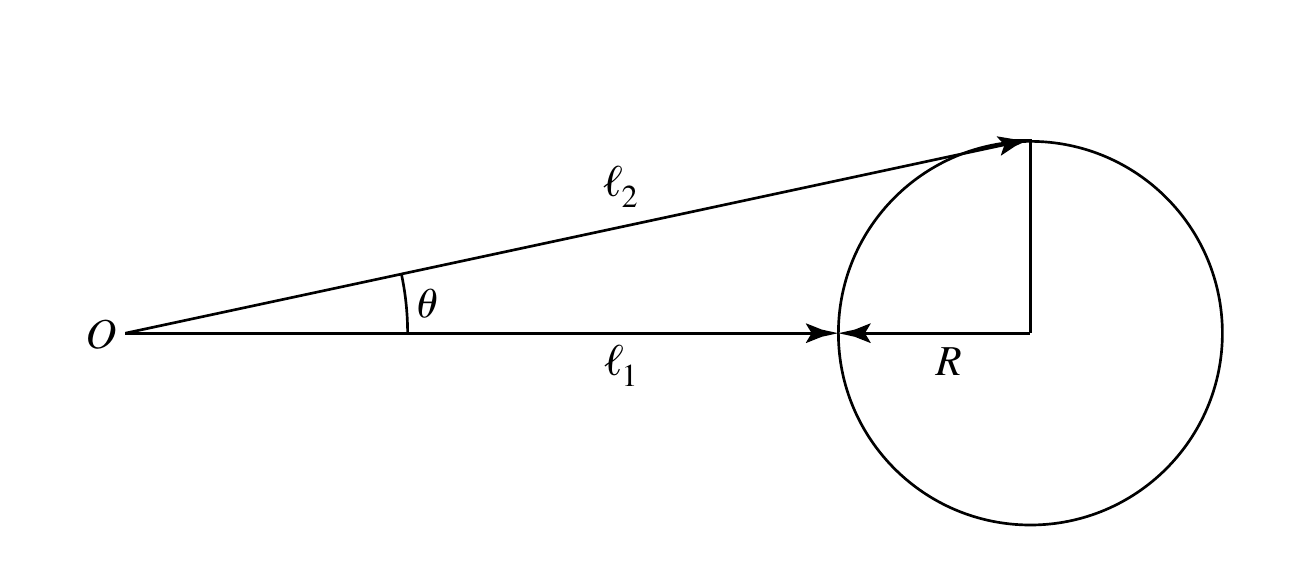
\includegraphics[scale= 0.2]{Figures/SizeView1.png}
 \caption{Διαδρομή φωτός από σφαιρικά συμμετρική πηγή. (Εικόνα από \cite{carroll_ostlie_2017})}
 \label{fig:lightpathsphere}
 \end{center}
\end{figure}
Για οπτικά πυκνή σφαίρα ακτίνας $R$ (σχήμα \ref{fig:lightpathsphere}) που υφίσταται σύντομη (στιγμιαία) αλλαγή στην λαμπρότητά της ακαριαία (στο σύστημα ηρεμίας της) και σε όλη την έκτασή της, μακρυνός παρατηρητής ($O$) καταλαβαίνει την μεταβολή αυτή από την διαφορά λαμπρότητας στο σήμα που δέχεται αρχικά από την εγγύτερη περιοχή, δηλαδή το σήμα που έχει διανύσει απόσταση $\ell_1$ , με τελευταίο σήμα το σήμα από το χείλος που διήνυσε απόσταση $\ell_2$ . Θα ισχύει
$$\ell_2 = \dfrac {\ell_1+R}{cos\theta} \simeq \ell_1+R$$
για $R<<1 $ και $cos \theta \simeq 1$, το ηλεκτρομαγνητικό σήμα από το χείλος της σφαίρας θα έχει διανύσει απόσταση μεγαλύτερη του κοντυνότερου σημείου κατά $\ell_2 - \ell_1 \simeq R$. \\
Έτσι η στιγμιαία αλλαγή στην λαμπρότητα αποτυπωνεται σε σήμα που διαρκεί $\Delta t = R/c$. Δηλαδή η διάρκεια αλλαγής στην λαμπρότητα μπορεί να χρησιμοποιηθεί για να θέσει ένα άνω όριο στις διαστάσεις της πηγής (για σφαιρικά-ισοτροπικά αντικείμενα).
Αν το σφαιρικό αυτό αντικείμενο απομακρυνόταν από τον παρατηρητή (Γη) με ταχύτητα $v$, η ακτίνα του στο σύστημα ανάφοράς μας (Γη) θα ήταν \cite{carroll_ostlie_2017}
\begin{equation}R = c\Delta t \sqrt{1-\dfrac{v^2}{c^2}}= \dfrac {c\Delta t }{\gamma} \label{eq:Radius}\end{equation}

\subsection*{Μάζα}

Για σφαιρικά συμμετρικό αντικείμενο σε ισορροπία η φωτεινότητα $L$ έχει άνω όριο το όριο \textlatin{Eddington} $ L < L_{Edd}$, όπου 
\begin{equation} L_{Edd} \approx 1.3 \cdot 10^{38} \big( \frac{M}{M_{\odot}} \big) \; erg \; s^{-1} \label{eq:Eddington}\end{equation}
Η $ L_{Edd}$ προκύπτει για υδροστατική ισορροπία όπου η πίεση είναι κυρίως πίεση ακτινοβολίας και η ύλη πλήρως ιονισμένο υδρογόνο και αποτελεί άνω όριο διότι η σφαιρική πρόσπτωση ύλης υπερισχύει της ακτινοβολίας ώστε να έχουμε σφαιρική προσαύξηση.\\
Για δεδομένη φωτεινότητα $L$, το άνω όριο μάζας από την σχέση \ref{eq:Eddington} gia $ L < L_{Edd}$ \cite{carroll_ostlie_2017}:
\begin{equation} M< \dfrac {L}{1.3\cdot 10^{38} \; erg \; s^{-1}} M_{\odot} \end{equation}
Ένα τέτοιο ποσό μάζας σε αυτές τις διαστάσεις είναι ένδειξη υπερμεγέθους μελανής οπής.
Η μάζα μελανής οπής ακτίνας $R$ από την σχέση ακτίνας \textlatin{Schwarzschild} και την σχέση \ref{eq:Radius}:
\begin{equation} M = \dfrac{Rc^2}{2G} =\dfrac {c^3\Delta t}{2G \gamma }  \end{equation}
Υπάρχουν κι άλλοι τρόποι να εκτιμήσουμε την μάζα της κεντρικής μελανής οπής, όπως η αστρική κατανομή και η δραστηριότητα σε μη-ενεργούς γαλαξίες, και έχουν να κάνουν με τον τρόπο με τον οποίο η μάζα αυτή επηρεάζει αέρια και αστέρες στο γαλαξιακό περιβάλλον\cite{AccrPower}.\\
Η άμεση παρατήρηση της κατανομής ταχυτήτων αστέρων και νεφών που αλληλεπιδρούν βαρυτικά τόσο μεταξύ τους όσο και με την κεντρική μελανή οπή σε κοντινούς γαλαξίες μπορεί να μας βοηθήσει να βγάλουμε συμπεράσματα για την κατανομή μάζας στην κεντρική περιοχή (για σφαιρική κατανομή μάζας $Μ$ με ακτίνα $r$ το θεώρημα \textlatin{virial} προβλέπει κατανομή ταχυτήτων $\overline{v}^2 \approx G M /r$ , αν υποθέσουμε ότι η δυναμική οφείλεται σε βαρυτικά φαινόμενα κυρίως και όχι π.χ. σε μαγνητικά). Παρατηρήσεις ταχυτήτων στην κεντρική περιοχή γαλαξιών είναι συνεπείς με την παρουσία υπερμεγέθους μελανής οπής σε κάθε γαλαξία.\\
Παρατηρείται συνέχεια στις ιδιότητες διαφορετικών κατηγοριών \textlatin{AGN} τόσο από υπέρλαμπρους \textlatin{AGN} σε χαμηλής λαμπρότητας (μεχρι και $10^{39}$ \textlatin{erg s}$^{-1}$) \textlatin{AGN} όσο και από ραδιογαλαξίες με ισχυρές διευρυμένες φασματικές γραμμές σε οπτικά μη-ενεργές ραδιοπηγές, αλλά ακόμα και στον Γαλαξία μας (με ραδιο-φωτεινότητα $\sim 10^{34}$ \textlatin{erg s}$^{-1}$). Τα παραπάνω είναι ενδείξεις ότι πιθανώς η ασθενής δραστηριότητα που παρατηρούμε σε μη-ενεργούς γαλαξίες είναι κατάλοιπο ενός <<νεκρού>> \textlatin{AGN}. Αυτό θα μας επέτρεπε να βγάλουμε συμπεράσματα για την μάζα της κεντρικής περιοχής ενεργών γαλαξιακών πυρήνων, αν γενικεύσουμε σχέσεις μάζας που παρατηρούμε σε κοντινούς μη-ενεργούς γαλαξίες.

\begin{figure*} 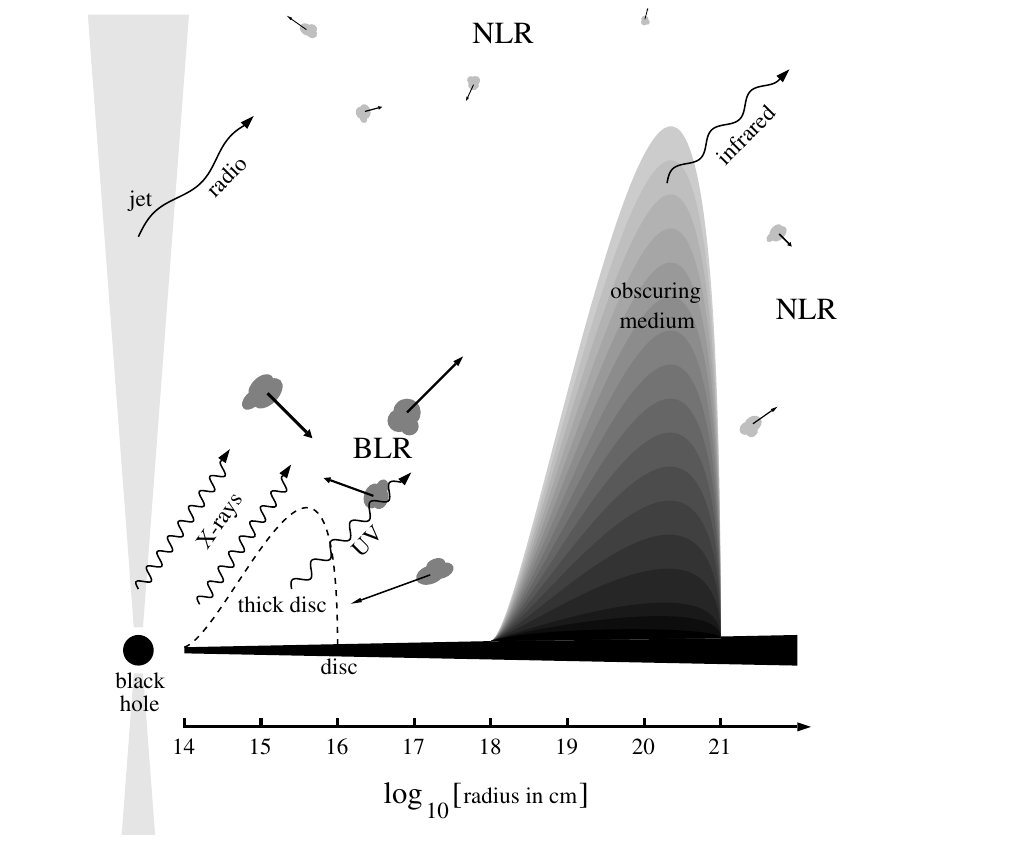
\includegraphics[width=1.2\linewidth]{Figures/AGNstucture.png} \caption{Δομή των \textlatin{AGN} που σχηματικά περιλαμβάνει στοιχεία που προτείνονται από ένα ενοποιητικό μοντέλο. Η διακεκομμένη γραμμή δείχνει πώς μπορεί να σχηματιστεί αδρός δίσκος. Το μέσο σκίασης \textlatin{(obscuring medium)} μπορεί να είναι τόρος σκόνης ή στρεβλωμένος δίσκος. \textlatin{BLR} είναι η περιοχή ευθείες παρατηρήσεις της οποίας μας δίνουν ευρείες φασματικές γραμμές εκπομπής, ενώ \textlatin{ΝLR} είναι η περιοχή ευθείες παρατηρήσεις της οποίας μας δίνουν στενές φασματικές γραμμές εκπομπής. (Εικόνα από \cite{AccrPower})}\label{fig:AGNstructure} \end{figure*}

\section{Μοντέλο μελανής οπής και δίσκου προσαύξησης}

Οι παραπάνω παρατηρήσεις- τα φάσματα εκπομπής και απορρόφησης, τα μεγέθη των παρατηρούμενων λαμπροτήτων, οι παρατηρούμενες χρονικές κλίμακες, οι θεμελιώδεις φυσικές αρχές- μας οδηγούν στο συμπέρασμα ότι η δομή των \textlatin{AGN} πρέπει να περιλαμβάνει παραγωγή ενέργειας σε μια μικρή συμπαγή περιοχή γυρω από αντικείμενο με πολύ μεγάλη μάζα.

Οι υπερμαζικές μελανές οπές είναι ευσταθείς και μπορούν να εκπέμψουν ισχυρή ακτινοβολία μέσω προσάυξησης στους \textlatin{AGN} πολύ αποδοτικά. Το πλέον καθιερωμένο μοντέλο για ενεργούς γαλαξιακούς πυρήνες είναι αυτό της υπερμαζικής μελανής οπής με δίσκο προσαύξησης (σχήμα \ref{fig:AGNstructure}). Το υλικό που ενεργοποιεί την προσαύξηση παρέχεται είτε από τοπικά αστρικά σμήνη είτε από το συνολικό αέριο και σκόνη του γαλαξία στου οποίου το κέντρο βρίσκεται\cite{AccrPower}. 
Η ύπαρξη τέτοιων μελανών οπών υποστηρίζεται και από την γενική σχετικότητα έναντι άλλων θεωριών (όπως π.χ. πυκνά σμήνη μαζικών αστέρων που σύντομα εξελίσονται σε υπερκαινοφανείς, υπερμαζικοί ασταθείς αστέρες) για τον μηχανισμό και την κεντρική περιοχή των \textlatin{AGN}\cite{AccrPower}.

\subsection{Κεντρική μελανή οπή}

Μια θεωρία βαρύτητας μας δίνει εξισώσεις κίνησης σωματίων που υφίστανται την βαρυτική επιροή σωμάτων με μεγάλη αδράνεια. Στην νευτώνεια θεώρηση, η ακτινική θέση $r(t)$ σωματίου σε τροχιά γύρω από σφαιρικά συμμετρικό μαζικό αντικείμενο μάζας $Μ$ δίνεται από την εξίσωση ενέργειας:
\begin{equation}
    \dfrac{1}{2} \Big( \dfrac{dr}{dt} \Big)^2 + V(r) = E
\end{equation}
Όπου $Ε$ σταθερή ενέργεια ανά μονάδα μάζας του σωματιδίου και 
\begin{equation}
    V(r)=h^2/2r^2- GM/r
\end{equation}
το ενεργό δυναμικό ανά μονάδα μάζας σωματίου με στροφορμή $h$.\\
Στην γενική σχετικότητα όλη η ενέργεια συνεισφέρει στην βαρυτική μάζα ενός συστήματος, συμπεριλαμβανομένου και της βαρυτικής δυναμικής ενέργειας. Ένα βαρυτικό πεδίο είναι ισχυρό όταν $GM m/r \sim mc^2$ gia σωμάτιο μάζας $m$, δηλαδή όταν η βαρυτική δυναμική ενέργειά του είναι της τάξης της ενέργειας μάζας ηρεμίας του. Για σφαιρικά συμμετρικό στάσιμο σώμα μάζας $Μ$ στο κενό η εξίσωση ενέργειας δίνεται από την λύση \textlatin{Schwarzschild}: 
\begin{equation}
    \dfrac{1}{c^2} \Big( \dfrac{dr}{d\tau} \Big)^2 + V^2(r) = E^2 \label{eq:SchwarzEnergy}
\end{equation}
Όπου $\tau$ ο ιδιόχρονος του σωματίου, η σχέση του οποίου με τον χρόνο $t$ του συστήματος συντεταγμένων είναι: 
\begin{equation}
    \dfrac{dt}{d\tau}  = E \Big(1 - \dfrac{2GM}{rc^2}  \Big)^{-1} \label{eq:SchwarzPropertime}
\end{equation}
Και το ενεργό δυναμικό στην περίπτωση αυτή είναι:
\begin{equation}
    V^2(r) =  \Big( 1 - \dfrac{2GM}{rc^2}  \Big)   \Big( 1 + \dfrac{h^2}{r^2c^2}  \Big) \label{eq:SchwarzPotential}
\end{equation}
Όπου  $h$ η σταθερή σχετικιστική στροφορμή ανά μονάδα μάζας του σωματίου που βρίσκεται σε τροχιά.\\
Καθώς η ακτινική απόσταση του σωματίου μικραίνει πλησιάζοντας την ακτίνα  \textlatin{Schwarzschild} του κεντρικού σώματος $ r \rightarrow 2GM/c^2 = R_S$ οι εξισώσεις \ref{eq:SchwarzPotential} kai \ref{eq:SchwarzPropertime} δείχνουν ότι $V \rightarrow 0$ kai $dt/d\tau \rightarrow \infty$. Για συμπαγή αντικείμενα μάζας $Μ$ η ακτίνα \textlatin{Schwarzschild} έχει φυσικό νόημα (ένα σωμάτιο μπορεί να φτάσει στην απόσταση αυτή χωρίς να ανακόπτεται από τις διαστάσεις του σώματος $Μ$) και είναι σημαντική αφού ορίζει τον ορίζοντα της μελανής οπής. Από την σχέση \ref{eq:SchwarzEnergy}, προκειμένου να ισχύει $(dr/d\tau)^2 \geq 0$, το ενεργό δυναμικό έχει ανώτατο όριο $V^2 \leq E^2$ και κατώτατο όριο το $Ω^2 \geq 0$ στην ακτίνα \textlatin{Schwarzschild}. 
Η σχέση \ref{eq:SchwarzPotential} επιτρέπει τροχιές σε αυτά τα όρια στο ενεργό δυναμικό μόνο για $ h \geq 2\sqrt{3} GM/c^2$, έτσι σωμάτια με στροφορμή $ h < 2\sqrt{3} GM/c^2$ δεν διαφέυγουν της μελανής οπής. Ευσταθείς τροχιές έχουμε για ελάχιστα της συνάρτησης $V(r)$, και συγκεκριμένα για
\begin{equation}
    r =  \frac{GM}{2c^2} \big[ H^2 - \sqrt{H^4 - 12H^2}     \big]
\end{equation}
Όπου $ H = c^2 h/GM$, με $ h \geq 2\sqrt{3} GM/c^2$. Η μικρότερη ακτίνα ευσταθούς τροχιάς γύρω από μελανή οπή \textlatin{Schwarzschild} ορίζεται $r_{min} = 6GM/c^2$ και ορίζει την επιφάνεια της μέγιστης δυνατής παραγωγής ενέργειας από τα προσπίπτοντα σωματίδια. Αφού σωμάτια που βρίσκονται από το κέντρο της μελανής οπής μέχρι την ελάχιστη αυτή ακτίνα ευσταθούς τροχιάς θα καταρεύσουν προς την μελανή οπή, σωματίδια που βρίσκονται οριακά σε απόσταση $r_{min}$ θα έχουν τον μεγαλύτερο χρόνο κατάρευσης και συνεπώς ακτινοβολίας\cite{AccrPower}.\\
Νευτώνειοι υπολογισμοί της μέγιστης αποδοτικότητας παραγωγής ενέργειας ως το πηλίκο της μέγιστης διαθέσιμης βαρυτικής δυναμικής ενέργειας προς την ενέργεια μάζας ηρεμίας δίνουν κατά προσέγγυση για μελανές οπές \textlatin{Schwarzschild}:
\begin{equation}
    \varepsilon_{max}  =  \frac{GMm/ 2 r_{min}}{mc^2} = \frac{1}{12}
\end{equation}
Για περιστρεφόμενες μελανές οπές με αξισυμμετρία στον άξονα στροφορμής μάζας $Μ$ και στροφορμής ανά μονάδα μάζας $Η$ στο κενό, η εξίσωση ενέργειας δίνεται από την λύση \textlatin{Kerr}. Για να περιγράψουμε τις μελανές οπές \textlatin{Kerr} ορίζουμε τις ποσότητες μήκους: $m = GM/c^2$ kai $\alpha = H/c$. Για τον ορίζοντα μελανών οπών \textlatin{Kerr} έχουμε διπλή λύση $r_{\pm} = m \pm \sqrt{(m^2-\alpha^2) }$ και η εξωτερική ακτίνα ορίζοντα είναι η $r_{+} = m + \sqrt{(m^2-\alpha^2) }$. Το ενεργό δυναμικό της κίνησης σε ισημερινό πεδίο μπορεί να οριστεί ως η ελάχιστη ενέργεια ανά μονάδα μάζας $E_{min}$ για την οποία η κίνηση είναι εφικτή σε ακτίνα $r_{+}$ και δίνεται από την σχέση:
\begin{equation} 
\begin{aligned}
V(r) \equiv E_{min}(r) =  {} &  \Big[\sqrt{r^2 - 2mr + \alpha^2} \sqrt{r^2h^2+ \big[r(r^2+ \alpha^2)+2 \alpha^2m \big]r}  +\\
& + 2 \alpha h m\Big] \Big[ r(r^2+ \alpha^2)+2 \alpha^2m \Big]^{-1}
\end{aligned}
\end{equation} 
Η μικρότερη ακτίνα ευσταθούς κυκλικής τροχιάς σωματίου γύρω από μελανή οπή \textlatin{Kerr} υπολογίζεται:
\begin{equation}
r_{min} = m \big[ 3 + A_2 \mp \sqrt{ (3-A_1)(3+A_1+2A_2) } \big]
\end{equation} 
Όπου $A_1 = 1+(1 - \alpha^2 /m^2)^{1/3} \big[ (1+\alpha/m)^{1/3} +(1- \alpha m)^{1/3}  \big]$, $A_2 = (3\alpha^2/m^2 + A_1^2)^{1/2}$, ενώ η σχέση έχει <<$-$>> για σωμάτια με τροχιά ομόρροπη της περιστροφής της μελανής οπής και <<$+$>> για σωμάτια με τροχιά αντίρροπη. 
Η επιφάνεια που ορίζει η μικρότερη ευσταθής ακτίνα αντιστοιχεί σε μέγιστη απόδοση παραγωγής ενέργειας\cite{AccrPower}:
\begin{equation}
\varepsilon_{max} = 1- \dfrac{r_{min} - 2m \pm (\alpha \sqrt{m}/ \sqrt{r_{min}})  } {\sqrt{ r_{min} - 3m \pm \big( 2\alpha \sqrt{m}/ \sqrt{r_{min}}\big)  }}
\end{equation}
Η απόδοση αυτή φτάνει το $40\%$ για σωμάτια με τροχιά ομόρροπη της περιστροφής της μελανής οπής και στροφορμή τέτοια ώστε $\alpha = m$. 

\subsection{Προσαύξηση}

\subsubsection*{Παροχή μάζας}

Τα περισσότερα μοντέλα ενεργών γαλαξιακών πυρήνων απαιτούν μεγάλη ποσότητα ύλης για την παραγωγή ενέργειας στην κεντρική περιοχή. Η προσάυξηση σε υπερμεγέθεις μελανές οπές είναι το κυρίαρχο και καθιερωμένο μοντέλο και απαιτεί συνεχή παροχή μάζας για την παραγωγή της παρατηρούμενης ενέργειας ακτινοβολίας. Προκειμένου να επιτευχθεί προσαύξηση, υλικό που βρίσκεται κοντά στην κεντρική μελανή οπή θα πρέπει να χάνει στροφορμή από την περιστροφή του ώστε να προσπίπτει στο κέντρο. Αυτό θα πρέπει να γίνεται με κάποιον αποδοτικό μηχανισμό και σε χρονικές κλίμακες που είναι τυπικές της γαλαξιακής εξέλιξης\cite{netzer_2013}. Το ζήτημα της παροχής μάζας (δηλαδή αερίου) έχει να κάνει τόσο με την προέλευση του αερίου όσο και με τον μηχανισμό με τον οποίο καταλήγει στην κεντρική περιοχή ώστε να χρησιμοποιηθεί ως υλικό προσαύξησης και να καταστήσει τον γαλαξιακό πυρήνα <<vενεργό>>. Έχουμε δύο περιπτώσεις προέλευσης του υλικού προσαύξησης στο καθιερωμένο μοντέλο των \textlatin{AGN}: στην πρώτη περίπτωση το υλικό προέρχεται από μια <<τοπική>> πυρηνική περιοχή (πυκνά νέφη ή αστρικά σμήνη σε ακτίνα μικρότερη των $10$ \textlatin{pc}), στην δεύτερη περίπτωση το υλικό προέρχεται από το κυρίως σώμα του γαλαξία, από διαγαλαξιακό μέσο ή από αλληλεπιδράση με άλλον γαλαξία (αέριο σε ακτίνα μεγαλύτερη του $1$ \textlatin{kpc})\cite{AccrPower}.

Όσον αφορά την περίπτωση πυρηνικού υλικού ως τροφοδότη της προσαύξησης, αν υποθέσουμε ότι το υλικό αυτό είναι αέριο και πυκνά αστρικά σμήνη, θεωρείται ότι περίπου $10^{9}$ αστέρες συγκενρώνονται σε ακτίνα $\sim 10 \; pc$ από το κέντρο του γαλαξία λόγω δυναμικών διαδικασιών που οφείλονται σε αστέρες και αέρια. Στην υπόθεση αυτή, παρακάμπτεται το πρόβλημα της μείωσης στροφορμής του υλικού, αφού αν έχει διαμορφωθεί αστρικό σμήνος στην περιοχή έχει ήδη μειωμένη στροφορμή. Όμως ακόμα κι αν έχουμε αστρικά σμήνη στην κεντρική περιοχή, ο ρυθμός με τον οποίο εκλύεται υλικό από διαδικασίες αστρικής εξέλιξης (παλιρροϊκές διαταραχές, συγκρούσεις αστέρων, αστρικός άνεμος) δεν είναι αρκετός για να παρέχει το απαιτούμενο υλικό προσαύξησης των λαμπρότερων \textlatin{AGN} που παρατηρούμε \cite{AccrPower}. \\
Αστέρες οι τροχιές των οποίων τους οδηγούν πολύ κοντά στην υπερμαζική μελανή οπή στο κέντρο του σμήνους διαλύονται από παλιρροϊκες δυνάμεις. Η εξέλιξη ενός τέτοιου σμήνους εξαρτάται από τον δυναμικό χρόνο $t_{dyn}$ (χρόνος αποκατάστασης δυναμικής ισορροπίας σε τροχιές) και τον χρόνο χαλάρωσης συστήματος δύο σωμάτων $t_{R}$ (χρόνος εκτροπής σώματος από το πεδίο βαρύτητας). Ο ρυθμός έκλυσης αερίου από παλιρροϊκές διαταραχές  
περιορίζεται από τον ρυθμό με τον οποίο οι αστρικές τροχιές μεταπίπτουν σε έναν κώνο 
ημι-ανοίγματος $\theta_{crit} \sim t_{dyn}/t_{R} $ γύρω από την διεύθυνση ακτινικής ταχύτητας λόγω απώλειας ενέργειας και στροφορμής. Ο μέγιστος ρυθμός έκλυσης αερίου για σφαιρικό αστρικό σμήνος με σχεδόν ισοτροπική κατανομή ταχυτήτων είναι της τάξης της μάζας του σμήνους προς τον χρόνο χαλάρωσης ή της τάξης μίας αστρικής μάζας προς δυναμικό χρόνο: αυτός ο ρυθμός δεν είναι αρκετός για να εξηγήσει τις μεγαλύτερες παρατηρούμενες λαμπρότητες μέσω ακτινοβολίας προσαύξησης, εκτός αν υπάρχει κάποιος μηχανισμός που ωθεί τους αστέρες σε μεγάλο αριθμό συγκρούσεων μεταξύ τους ώστε να υπάρξει απελευθέρωση μεγαλύτερης μάζας. Επίσης, όταν η κεντρική υπερμεγέθης μελανή οπή ξεπεράσει τις $\sim 10^8$ M$_\odot$, οι παλιρροϊκές δυνάμεις δεν είναι πλέον ικανές να διαλύσουν έναν αστέρα πριν αυτός καταρεύσει στην μελανή οπή- όταν ο αστέρας καταρρέει χωρίς να διαλυθεί, αυτό γίνεται με σχετικά μικρή απώλεια ενέργειας σε ηλεκτρομαγνητική ακτινοβολία\cite{AccrPower}. \\
Πυκνά αστρικά σμήνη όπως αυτά που περιγράψαμε δεν μπορούν να σχηματιστούν ως αποτέλεσμα δυναμικής χαλάρωσης βαρυτικά αλληλεπιδρώντων σωμάτων (στο πρότυπο των δύο σωμάτων), αφού θα κατέληγαν σε μικρό πυρήνα αστέρων με πολύ μεγάλες ταχύτητες που θα διαλύονταν από συγκρούσεις\cite{AccrPower}. Έτσι, αν επικεντρωθούμε σε δυναμική αερίων, πρέπει να υπάρχει μηχανισμός που συγκεντρώνει το διαθέσιμο αέριο από μια αρχικά μεγάλη περιοχή σε μικρό όγκο και να εξηγεί την απώλεια στροφορμής ώστε να προσπίπτει προς προσαύξηση. %Οι τοπικοί μηχανισμοί, όπως είδαμε ακόμα κι αν πυκνά αστρικά σμήνη διατίθενταν στην πυρηνική περιοχή του γαλαξία, δεν επαρκούν. 

Παρατηρήσεις υποδεικνύουν ότι εκτός του γαλαξιακού πυρήνα υπάρχουν μεγάλα ποσά αερίου υπό μορφή διαστρικού μέσου, οπότε εξετάζουμε τον μηχανισμό που μπορεί να μεταφέρει τα αέρια αυτά μέσω τυρβώδους ιξώδους ροής όπως στο μοντέλο $\alpha-$δίσκων που θεωρείται ότι λειτουργεί για την μεταφορά μάζας και προσαύξηση σε διπλά αστρικά συστήματα αστέρα-μελανής οπής. Στο μοντέλο αυτό ($\alpha-$δίσκων) θεωρούμε ότι το αέριο έχει ιξώδες $\eta = \alpha c_s H$, όπου $c_s$ η ταχύτητα του ήχου, $H$ η κλίμακα ύψους του δίσκου και $\alpha$ παράμετρος προσαύξησης ($\alpha=0$ όταν δεν έχουμε προσαύξηση). Για συμβατικές παραδοχές της φυσικής κατάστασης του αερίου και με παράμετρο προσάυξησης $\alpha \leq 1$ μια απλή εκτίμηση δίνει χρόνο ροής προς την πυρηνική περιοχή $10^9$ \textlatin{yr} για αέριο που βρίσκεται σε ακτίνα μεγαλύτερη των $10$ \textlatin{pc} \cite{AccrPower}. Έτσι, ένας συμβατικός δίσκος προσαύξησης στο μοντέλο αυτό δεν μπορεί να παρέχει σταθερά υλικό προσαύξησης στην πυρηνική περιοχη. Έπειτα, οι λεπτοί δίσκοι προσαύξησης (που αποδίδουν μεγαλύτερη λαμπρότητα στο μοντέλο αυτό) είναι βαρυτικά ασταθείς σε μεγάλες ακτίνες όπου είναι πιο εύκολο να ψυχθούν κατά περιοχές και οι ψυχρές περιοχές να αποσυζευχθούν οδηγώντας σε επιβράδυνση της προσαύξησης.\\
Στο πρότυπο των $\alpha-$δίσκων, λοιπόν, δεν μπορεί να διατηρηθεί θερμή ροή προσαύξησης με τα συμβατικά χαρακτηριστικά που αναφέραμε, οπότε χρειαζόμαστε έναν μηχανισμό με ενεργό παράμετρο προσαύξησης $\alpha \gg 1$. Έχουν προταθεί μηχανισμοί που θα μπορούσαν να αποδόσουν $\alpha \gg 1$ με σύζευξη ρευστού σε πολύ διαφορετικές ακτινικές κλίμακες. Δύο τέτοιοι μηχανισμοί είναι μαγνητικά πεδία γαλαξιακής κλίμακας και μη αξισυμμετρικές βαρυτικές αστάθειες. Αν ένα μεγάλης κλίμακας πολοειδές μαγνητικό πεδίο υπήρχε σε γαλαξίες που <<φιλοξενούν>> υπερμεγέθη μελανή οπή, οι μαγνητοϋδροδυναμικές ροπές που γενά η στρέψη του πεδίου θα μπορούσαν να συζεύξουν αέριο σε διαφορετικές ακτινικές κλίμακες και να μεταφέρουν υλικό προς το κέντρο μειώνοντας την στροφορμή του\cite{AccrPower}. Σε αυτήν την διαδικασία δημιουργούνται τοροειδή πεδία που αυξάνουν την μαγνητική πίεση και παραλληλίζουν την εκροή ύλης με τον άξονα περιστροφής εξηγώντας παρατηρούμενους πίδακες. %Ενδείξεις τέτοιων μανητικών πεδίων υπαρχουν για τον Γαλαξία μας και σε κάποιους κοντινούς γαλαξίες, χωρίς όμως να είναι ξεκάθαρο αν η έντασή τους είναι αρκετή.   
Ένας άλλος προτεινόμενος μηχανισμός είναι μη αξισυμμετρικές δομές (όπως ράβδοι από αστέρες και αέριο, ελλειψοειδείς δίσκοι και δακτύλιοι, γαλαξίες-συνοδοί) και διαταραχές που προκαλούνται από παλιρροϊκές αλληλεπιδράσεις με άλλους γαλαξίες ή συγχωνεύσεις με άλλους γαλαξίες. Η αρχή λειτουργίας του μηχανισμού αυτού είναι ότι καθώς αέριο περιστρέφεται γρηγορότερα από την ράβδο του γαλαξία, πλησιάζοντάς την επιταχύνεται προς το ελάχιστο του βυθίσματος δυναμικού κι έπειτα επιβραδύνεται και συμπιέζεται καθώς προπερνά την ράβδο. Το ωστικό κύμα του αερίου στην μπροστινή όψη της ράβδου (που οδηγεί την κίνηση) χάνει στροφορμή την οποία παρέχει στην ράβδο με αποτέλεσμα να ρέει προς το κέντρο. Παρόμοια ροή αερίου θα έχουμε για διαταραχές που προκαλούνται από αλληλεπίδραση  με άλλους γαλαξίες όπου προκύπτουν δομές σαν ράβδοι. Ακόμα, όμως, και σε αύτην την περίπτωση το αέριο δεν ρέει μέχρι το κέντρο, αφού όσο μια μάζα αερίου προχωρά προς το κέντρο τόσο ασθενεί η επίδραση της ράβδου. Το αέριο τυπικά φθάνει μέχρι ακτίνα $\sim 1$ \textlatin{pc} όπου ούτε η ιξώδης ροή δεν αρκεί για να το μεταφέρει με ικανοποιητικό ρυθμό προς το κέντρο, όμως αν η ίδια η μάζα του αερίου που συσσωρεύεται γίνει δυναμικά σημαντική μπορεί να έχουμε μη-αξισυμμετρικές δυναμικές αστάθειες και ανακατανομή στροφορμής που ωθεί το αέριο προς την κεντρική περιοχή\cite{AccrPower}.    

\subsubsection*{Δίσκος προσαύξησης}

Σε γαλαξιακές χωρικές και χρονικές κλίμακες, η παροχή υλικού προσαύξησης στις υπερμεγέθεις μελανές οπές εξαρτάται από μηχανισμούς όπως συγκρούσεις και συγχωνεύσεις γαλαξιών, δυναμικές αστάθεις όπως ράβδοι, μαγνητικά πεδία που φέρνουν υλικό σε αποστάσεις $1-10$ \textlatin{pc} από την κεντρική μελανή οπή. Σε κοντινότερες ακτινικές αποστάσεις ο μηχανισμός προσαύξησης βασίζεται στην βαρυτική έλξη της μελανής οπής, την ιδιοβαρύτητα του υλικού, την τοπική υδροδυναμική πίεση και πίεση ακτινοβολίας, αστρικούς ανέμους, υπερκαινοφανείς εκρήξεις, μαγνητικό και θερμικό ιξώδες του αερίου. Αέριο με χαμηλή στροφορμή προsπίπτει σφαιρικά στην μελανή οπή, ενώ αέριο με υψηλή στροφορμή προσπίπτει στην μελανή οπή μέσω κεντρικού δίσκου προσαύξησης που παρέχει έναν μηχανισμό ιξώδους ροής που μειώνει την στροφορμή\cite{netzer_2013}.
Η προσαύξηση ύλης με σημαντική στροφορμή σε μελανή οπή συνοδεύεται από σχηματισμό δίσκου από το υλικό πρασάυξησης. Τέτοιοι δίσκοι πρέπει να σχηματίζονται και σε μελανές οπές αστρικής προέλευσης και σε υπερμεγέθεις μελανές οπές.

Μοντέλα δίσκων προσαύξησης βασίζονται σε παρατηρήσεις μελανών οπών σε διπλά συστήματα και ο μηχανισμός προσαύξησης γενικεύεται για υπερμεγέθεις μελανές οπές. Για προσαύξηση σε μελανή οπή τα σύγχρονα μοντέλα προβλέπουν την ροή αερίου είτε σε λεπτούς δίσκους που περιστρέφονται γύρω από την μελανή οπή είτε ένα αδρό χαοτικό νέφος. Για φωτεινότητα ακτίνων Χ που υπερβαίνει το όριο \textlatin{Eddington} είναι πιο πιθανή η εικόνα του αδρού νέφους, ενώ για υπο-\textlatin{Eddington} φωτεινότητα η εικόνα του λεπτού δίσκου. Για φωτεινότητα χαμηλότερη της φωτεινότητας \textlatin{Eddington} ώστε $L \lesssim 10^{-2} L_{Edd}$ θερμικές αστάθειες λόγω χαμηλής οπτικής πυκνότητας μπορούν να διαταράξουν την εσωτερική περιοχή λεπτού δίσκου και να μεταπίψει σε αδρό νέφος, αλλά ακόμα και για φωτεινότητα $L\lesssim 10^{-4} L_{Edd}$ έχουμε ασταθείς λεπτούς δίσκους\cite{Lightman1974}. 

Σε ένα διαφορικά περιστρεφόμενο μέσο (όπως είναι το υλικό στον δίσκο πρσαύξησης) οι εφαπτομενικές τάσεις ανάμεσα στα διάφορα στρώματα (οι οποίες σχετίζονται με την ύπαρξη μαγνητικού πεδίου), η τυρβώδης ροή και το μοριακό και ηλεκτρομαγνητικό ιξώδες είναι οι μηχανισμοί που μεταφέρουν στροφορμή\cite{ShakuraBlackHoles} έτσι ώστε το υλικό να καταρεύσει σπειροειδώς προς το κέντρο. Η ενέργεια που χάνει το υλικό (αέριο) μπορεί να μετατραπεί σε ηλεκτρομαγνητική ακτινοβολία με πολύ μεγάλη απόδοση (είδαμε από 4\% έως 40\% για αντικείμενα \textlatin{Kerr}) ή μπορεί να μετατραπεί σε κινητική ενέργεια του αερίου με αποτέλεσμα να διαφύγει του δίσκου ή μπορεί να θερμάνει το αέριο με την θερμική ενέργεια να μεταφέρεται στην μελανή οπή (\textlatin{advection accretion flow})\cite{netzer_2013}.

Το πιο χρήσιμο μοντέλο δίσκων προσαύξησης είναι αυτό των $\alpha-$δίσκων, ένα νευτώνειο μοντέλο (περιγράφει καλά υλικό σε ακτίνα $R>3R_{Schw}$) που βασίζεται σε παρατηρήσεις μελανών οπών σε διπλά συστήματα και περιγράφει λεπτούς δίσκους. Στο μοντέλο αυτό παραδεχόμαστε τυρβώδη ροή, μη-γραμμικές διαταραχές (δηλαδή αλληλεπίδραση μεταξύ τυρβώδων παλμών) και ως αποτέλεσμα μια αυτο-συντηρούμενη τύρβη\cite{ShakuraBlackHoles}. 
Για μη-μηδενικά μαγνητικά πεδία στους δίσκους, αστάθειες διατμητικής τάσης συντηρούν επίσης τυρβώδη ροή η οποία είναι ο κυρίαρχος παράγοντας που μεταφέρει στροφορμή\cite{Blackman98}. \\
Η δομή και η ακτινοβολία στατικών δίσκων καθορίζονται από τρείς φυσικές παραμέτρους: την μάζα της μελανής οπής $Μ$, τον ρυθμό προσαύξησης $\dot M$ (ή την συνολική φωτεινότητα του δίσκου $L = \zeta \dot M c^2$, όπου $\zeta$ ο συντελεστής απόδοσης της παραγωγής ενέργειας) και την παράμετρο $\alpha$, η οποία χαρακτηρίζεται από το επίπεδο τυρβώδους ροής και από χαοτικά μικρής κλίμακας μαγνητικά πεδία\cite{ShakuraInstability}.
\begin{equation}
    \alpha = \dfrac{v_t l_t}{v_s Η} + \dfrac{B}{4\pi \rho v_s^2}
\end{equation}
Όπου $v_t$ kai $v_s$ η ταχύτητα τυρβώδους ροής και η θερμική ταχύτητα αντίστοιχα, $B^2/8\pi$ η ενεργειακή πυκνότητα του χαοτικού μαγνητικού πεδίου, $\rho v_s^2/2$ η θερμική ενεργειακή πυκνότητα του υλικού στον δίσκο, $l_t$ το μήκος τυρβώδους ανάμειξης και $Η$ το ημι-ύψος του δίσκου.\\
Η φωτεινότητα, όπως έχουμε δεί, φαινομενικά φράσσεται από την φωτεινότητα \textlatin{Eddington} $$L_{Edd} = 1.3\times10^{38} \Big(\dfrac{M}{M_\odot}   \Big) \; erg \; s^{-1}$$ 
η οποία προκύπτει εξισώνοντας την βαρυτική δύναμη με την δύναμη πίεσης ακτινοβολίας για πλάσμα στο εσωτερικό του δίσκου. Για φωτεινότητες κοντά στο όριο \textlatin{Eddington} $L/L_{Edd} \gtrsim \frac{1}{50} (M_\odot/\alpha M)^{1/8}$ ο δίσκος αποτελείται από τρείς περιοχές, την <<vεσωτερική>> ζώνη (ζώνη Α) όπου η πίεση ακτινοβολίας είναι μεγαλύτερη από την πίεση αερίου και η σκέδαση ελεύθερων ηλεκτρονίων κυριαρχεί σε σχέση με άλλες διαδικασίες απορρόφησης ακτινοβολίας. Αυτή η περιοχή εκπέμπει το μεγαλύτερο ποσό ενέργειας ακτινοβολίας του δίσκου και οι διαδικασίες \textlatin{Compton} καθορίζουν το παρατηρούμενο φάσμα. Σε μεγαλύτερη ακτίνα από την μελανή οπή βρίσκεται η ζώνη Β όπου η πίεση πλάσματος είναι μεγαλύτερη από την πίεση ακτινοβολίας, αλλά η σκέδαση ελεύθερων ηλεκτρονίων υπερισχύει στην διάδοση ακτινοβολίας. Πέρα από την ζώνη Β υπάρχει η ψυχρότερη περιοχή Γ όπου φαινόμενα απορρόφησης συμβάλουν στην οπτική πυκνότητα\cite{ShakuraInstability}.
Για $L/L_{Edd} < \frac{1}{50} (M_\odot/\alpha M)^{1/8}$  δεν έχουμε την ασταθή περιοχή Α. 

\subsection{Άλλα χαρακτηριστικά των \textlatin{AGN}}

Άλλα δομικά χαρακτηριστικά των \textlatin{AGN} πιθανώς υπάρχουν γύρω από την μελανή οπή και επηρεάζουν το φάσμα λόγω της θέσης τους, της πυκνότητας ύλης σε αυτά, του ιονισμού σε αυτά, της σύνθεσης ή ταχύτητάς τους (σχήμα \ref{fig:AGNstructure}). Θα εξετάσουμε μόνο μερικά από αυτά. 

\subsubsection*{Περιοχή διευρυμένων φασματικών γραμμών \textlatin{(Broad Line Region)}}
Πρόκειται για περιοχή με νέφη υψηλής χωρικής πυκνότητας σωματιδίων (\textlatin{n}$_{e} \sim 10^{10}$ \textlatin{cm}$^{-3}$) με μεγάλη επιφανειακή πυκνότητα (πυκνότητα στήλης) Ν$_{Η} \sim 10^{23}$ \textlatin{cm}$^{-2}$ γύρω από την υπερμεγέθη μελανή οπή και τον δίσκο προσαύξησης. Για πολύ λαμπρούς \textlatin{AGN} η περιοχή αυτή βρίσκεται σε ακτίνα $0.1-1$ \textlatin{pc} από την κεντρική μελανή οπή. Τα νέφη αυτά διατηρούνται για πολούς δυναμικούς χρόνους είτε επειδή είναι περιορισμένα είτε επειδή είναι μέλη μεγαλύτερων σωμάτων με ιδιοβαρύτητα (όπως π.χ. αστέρες). Η τυπική κεπλεριανή ταχύτητα τέτοιων νεφών είναι $ \sim 3000$ \textlatin{km s}$^{-1}$ kai αυτό αποτυπώνεται στα πλάτη των φασματικών γραμμών εκπομπής\cite{netzer_2013}.

\subsubsection*{Περιοχή στενών φασματικών γραμμών \textlatin{(Narrow Line Region)}}

Όπως φαίνεται και στο σχήμα \ref{fig:AGNstructure}, η περιοχή στενών φασματικών γραμμών είναι περιοχή με νέφη χαμηλότερης πυκνότητας (\textlatin{n}$_{e} \sim 10^{4}$ \textlatin{cm}$^{-3}$) με επιφανειακή πυκνότητα Ν$_{Η} \sim 10^{20-21}$ \textlatin{cm}$^{-2}$ γύρω από την υπερμεγέθη μελανή οπή. Η περιοχή αυτή βρίσκεται σε ακτίνα $> 3$ \textlatin{pc} από την κεντρική μελανή οπή για πολύ λαμπρούς \textlatin{AGN} και είναι πιο μαζική από την \textlatin{Broad Line Region}. Η τυπική ταχύτητα (αν θεωρήσουμε ότι τα νέφη αυτά βρίσκονται στο βαρυτικό πεδίο του γαλαξία) είναι της τάξης των $300$ \textlatin{km s}$^{-1}$. Το αέριο αυτό μπορεί να σχηματίσει διάφορες δομές, χρησιμοποιούμε τον όρο <<νέφος αερίων>> ως γενική περιγραφή\cite{netzer_2013}. 

\subsubsection*{Αέριο υψηλού ιονισμού}

Θεωρούμε ότι σε χωρική κλίμακα $0.1-10 $ \textlatin{pc} από το κέντρο υπάρχει περιοχή με επιφανειακή πυκνότητα Ν$_{Η} \sim 10^{21-23}$ \textlatin{cm}$^{-2}$ και πυκνότητα ικανή να παράξει ιονισμό 10-100 φορές υψηλότερο απ> ότι το αέριο sthn \textlatin{BLR} kai thn \textlatin{NLR.} Για το αέριο αυτό αναμένουμε ισχυρή απορρόφηση και εκπομπή στις ακτίνες Χ\cite{netzer_2013}.

\subsubsection*{Τόρος}
%Θα πρεπει ισως μα εξιγισεις οτι η υποθεση του τορου προερχεται απο την υπαρξη Ι/ΙΙ τυπου αντικειμενων, και η απλοικη υποθεση οτι υπαρχει υλικο σε μορφη τορου και η διαδοροποιηση αναμεσα σε Ι/ΙΙ ειναι καθαρα γεωμετρικο φαινομενο. 
Προκειμένου να εξηγηθεί η διαφοροποίηση μεταξύ \textlatin{AGN} τύπου Ι και τύπου ΙΙ ως γεωμετρικό φαινόμενο, θεωρούμε ότι υπάρχει τοροειδής δομή από αέριο, μοριακό αέριο και σκόνη σε περιοχή μεταξύ $0.1$ και $10$ \textlatin{pc} από την κεντρική μελανή οπή με πυκνότητα αερίου $\sim 10^{4}-10^{7}$ \textlatin{cm}$^{-3}$, επιφανειακη πυκνότητα που κυμαίνεται N$_{H} \sim 10^{22-24}$ \textlatin{cm}$^{-2}$ και κεπλεριανές ταχύτητες της τάξης των $1000$ \textlatin{km  s}$^{-1}$. Ο τόρος αυτός είναι οπτικά αδιαφανής για όλα τα μήκη κύματος εκτός του υπερύθρου και πιθανότατα σκιάζει την εκπομπή από τον δίκο προσάυξησης και την \textlatin{BLR} για παρατήρηση από ορισμένες διευθύνσεις\cite{netzer_2013}.

\subsection{Θεμελιώδη φυσικά μεγέθη συστήματος προσάυξησης}

\subsubsection*{Χαρακτηριστικές χρονικές κλίμακες}

Οι χαρακτηριστικοί χρόνοι μας δίνουν πληροφορίες για την συμπεριφορά ενός συστήματος. Για στατικούς, λεπτούς (δηλαδή ψυχρούς κεπλεριανούς) $\alpha-$δίσκους η μικρότερη χρονική κλίμακα είναι ο δυναμικός χρόνος (ο χρόνος ώστε να επέλθει δυναμική ισορροπίa)\cite{spruit2010accretion}
\begin{equation}
    t_{dyn} = \Big( \dfrac{GM}{r^3} \Big)^{-1/2}
\end{equation}
όπου $M$ η μάζα κεντρικής μελανής οπής και $r$ η απόσταση από αυτήν.\\
Η χρονική κλίμακα για την ακτινική μετακίνηση μέσα στον δίσκο για απόσταση $r$ είναι ο χρόνος ιξώδους
\begin{equation}
    t_{visc} = \dfrac{2f}{3 \alpha \Omega}   \Big( \dfrac{r}{H} \Big)^{2}
\end{equation}
όπου $f=1-\big(\frac{r_i}{r})^{1/2}$ με $r_i$ την εσωτερική ακτίνα του δίσκου, $H$ το ημι-ύψος του δίσκου και $\Omega$ η κεπλεριανή περιστροφή του δίσκου.\\
Οι θερμικές χρονικές κλίμακες είναι ο χρόνος ψύξης και ο χρόνος θέρμανσης. Αν $E_t$ η θερμική ενέργεια (ενθαλπία) του δίσκου ανά μονάδα επιφάνειας και $W_\eta=(9/4) \Omega^2 \eta \Sigma$ είναι ο ρυθμός θέρμασης λόγω ιξώδους διάχυσης (όπου $\eta$ το ιξώδες και $\Sigma$ η επιφανειακή πυκνότητα του δίσκου), τότε η χαρακτηριστική χρονική κλίμακα θέρμανσης
\begin{equation}
    t_{h} = \dfrac{E_t}{W_\eta}
\end{equation}
Ομοίως, ο χαρακτηριστικός χρόνος ψύξης
\begin{equation}
    t_{c} = \dfrac{E_t}{2 \sigma_r T_s^4}
\end{equation}
όπου η επιφανειακή θερμοκρασία εκφράζεται ως συνάρτηση μάζας κεντρικής μελανής οπής $M$ kai ρυθμού προσαύξησης $\dot M$ $$ \sigma_r T_s^4 = \dfrac{GM}{r^3} \dfrac{3\dot M}{8\pi} \Big[ 1-\big(\frac{r_i}{r})^{1/2}\Big]$$
Για λεπτούς δίσκους οι δύο αυτές κλίμακες συμπίπτουν, αφού η διάχυση ιξώδους ενέργειας ισορροπείται τοπικά από την ακτινοβολία του δίσκου από την διπλή επιφάνειά του. Σε αδρούς δίσκους \textlatin{ADAF (advection dominated accretion flow)} δεν υπάρχει αυτή η ισορροπία, αφού η μεταφορά \textlatin{(advection)} θερμότητας με την ροή προσαύξησης δεν είναι αμελητέα- τότε $t_c>t_h$ \cite{spruit2010accretion}.\\
Οι ακτίνες Χ παράγονται από διαδικασίες αντιστρόφου σκεδασμού \textlatin{Compton.} Η χρονική κλίμακα ψύξης (ελάτωσης ενέργειας) των θερμικών ηλεκτρονίων μέσω της αντίστροφης σκέδασης \textlatin{Compton} sτο μη-σχετικιστικό όριο ($\gamma \approx 1$) είναι
\begin{equation}
    t_{Compt} = \dfrac{6\pi G^2 m_e}{\sigma_T c^4} \dfrac{\xi ^2}{\zeta} \dfrac{M_{BH}^2}{\dot M} 
\end{equation}
Όπου $\xi$ η ακτινική απόσταση σε μονάδες ακτίνας \textlatin{Schwarzschild} $R=\xi R_{Schw}$ και $\zeta$ η απόδοση της διαδικασίας προσαύξησης, οπότε η λαμπρότητα των φωτονίων πρίν την σκέδαση (\textlatin{seed photons}) $L_{seed}=\zeta \dot{M} c^2$.
 
Παρατηρούμε ότι η χαρακτηριστική χρονική κλίμακα δυναμικού χρόνου εξαρτάται από την μάζα μελανής οπής $M$, ενώ οι χαρακτηριστικές χρονικές κλίμακες ιξώδους πρόσπτωσης και θερμικών διαδικασιών εξαρτώνται από την μάζα μελανής οπής και από την προσαύξηση, είτε με ευθεία εξάρτηση από τον ρυθμό προσάυξησης $\dot M$, είτε από τον όρο που μοντελοποιεί την τυρβώδη προσαύξηση  $\alpha$. Έτσι συμπεραίνουμε πως τα μεγέθη της μάζας μελανής οπής και του ρυθμού προσάυξησης είναι θεμελιώδεη για την συμπεριφορά του συστήματος προσαύξησης. 

\subsubsection*{Διαταραχές πρώτης τάξης στον δίσκο}

Η εφαρμογή της θεωρίας διαταραχών (έστω και πρώτης τάξης) για σύστημα προσαύξησης δεν είναι τετριμμένη διαδικασία. Η φυσική περιγραφή για σύστημα προσάυξησης στο απλό μοντέλο των $\alpha$-δίσκων απαιτεί\cite{ShakuraInstability} εξίσωση κεπλεριανής κίνησης, εξίσωση συνέχειας, εξίσωση διατήρησης ορμής, υδροστατική εξίσωση, εξίσωση τάσεων ιξώδους, εξίσωση παραγωγής ενέργειας λόγω τριβής, εξίσωση απώλειας ενέργειας λόγω ακτινοβολίας και καταστατική εξίσωση.

Αποτελέσματα εργασιών πάνω στην θεωρία μικρών γραμμικών διαταραχών στο πρότυπο της τυρβώδους προσαύξησης δίνουν τους εξής συσχετισμούς\cite{Blackman98} \\
Για λεπτούς $\alpha$-δίσκους:\\
\begin{equation}
    \frac{\Delta L_\nu}{L_\nu} \propto \alpha M_{BH}^{1/2} R^{3/4} \frac{H}{R}
\end{equation}

Για αδρούς \textlatin{ADAF} δίσκους:\\
\begin{equation}
    \frac{\Delta L_\nu}{L_\nu} \propto \alpha^2 M_{BH}^{1/2} R^{3/4} \frac{H}{R}
\end{equation}
Όπου $L_\nu$ η λαμπρότητα του δίσκου και $\Delta L_\nu$ διαταραχή σε αυτήν, $\alpha$ η παράμετρος τυρβώδους προσαύξησης, $R$ η ακτίνα του δίσκου, $M_{BH}$ η μάζα κεντρικής μελανής οπής και $H$ το ημι-ύψος του δίσκου.

Βλέπουμε, λοιπόν, πως και στην πρώτη προσέγγυση της θεωρίας διαταραχών η μάζα μελανής οπής και η παράμετρος προσαύξησης παίζουν σημαντικό ρόλο.





